\documentclass[aspectratio=169]{beamer}
\usepackage{tikz}
\usepackage{graphicx}
\usepackage{xypic}

\usecolortheme{whale}
\usetikzlibrary{er,positioning}  
\usetikzlibrary{decorations.pathreplacing}
\usetikzlibrary{arrows, decorations.markings}
\usetikzlibrary{shapes.geometric}
\usetikzlibrary{mindmap}

\setbeamertemplate{navigation symbols}{}

% \setbeameroption{show notes on second screen=right}

\definecolor{violet}{rgb}{0.53, 0.0, 0.69}

\definecolor{blue1}{RGB}{126,126,206}
\definecolor{blue2}{RGB}{87,87,192}
\definecolor{blue3}{RGB}{51,51,178}
\definecolor{blue4}{RGB}{27,26,107}

\tikzstyle{every link} = []
\tikzstyle{link} = [>=triangle 60, draw, every link]

\definecolor{attr}{RGB}{10,153,2}

\graphicspath{{img/}{./}} % Specifies where to look for included images (trailing slash required)

\newcommand<>{\red}[1]{\textcolor#2{red}{#1}}
\newcommand<>{\green}[1]{\textcolor#2{green}{#1}}
\newcommand<>{\gray}[1]{\textcolor#2{gray}{#1}}


\title{Bases de Datos Columnares}
\subtitle{}
\author[Garc\'ia L., Cardentey V. M., Ledesma. A]{
    Lic. Andy Ledesma Garc\'ia\\ 
    Lic. V\'ictor M. Cardentey Fundora\\ 
    Dra. C. Lucina Garc\'ia Hern\'andez
}
\institute[MATCOM-UH]{
    Departamento de Computaci\'on\\
    Facultad de Matem\'atica y Computaci\'on\\
    Universidad de La Habana\\[3mm]
    Licenciatura en Ciencia de Datos
}
\date[]{19 de marzo de 2024}


\begin{document}
    \maketitle
    
    \section{Almacenamiento basado en columnas}
    \begin{frame}
    \frametitle{Modelo de datos}

    \begin{block}{Estructura de datos}
        Cada par llave-valor es almacenado utilizando una estructura asociativa (p.e. \textit{hash table} o \textit{B tree}). 

        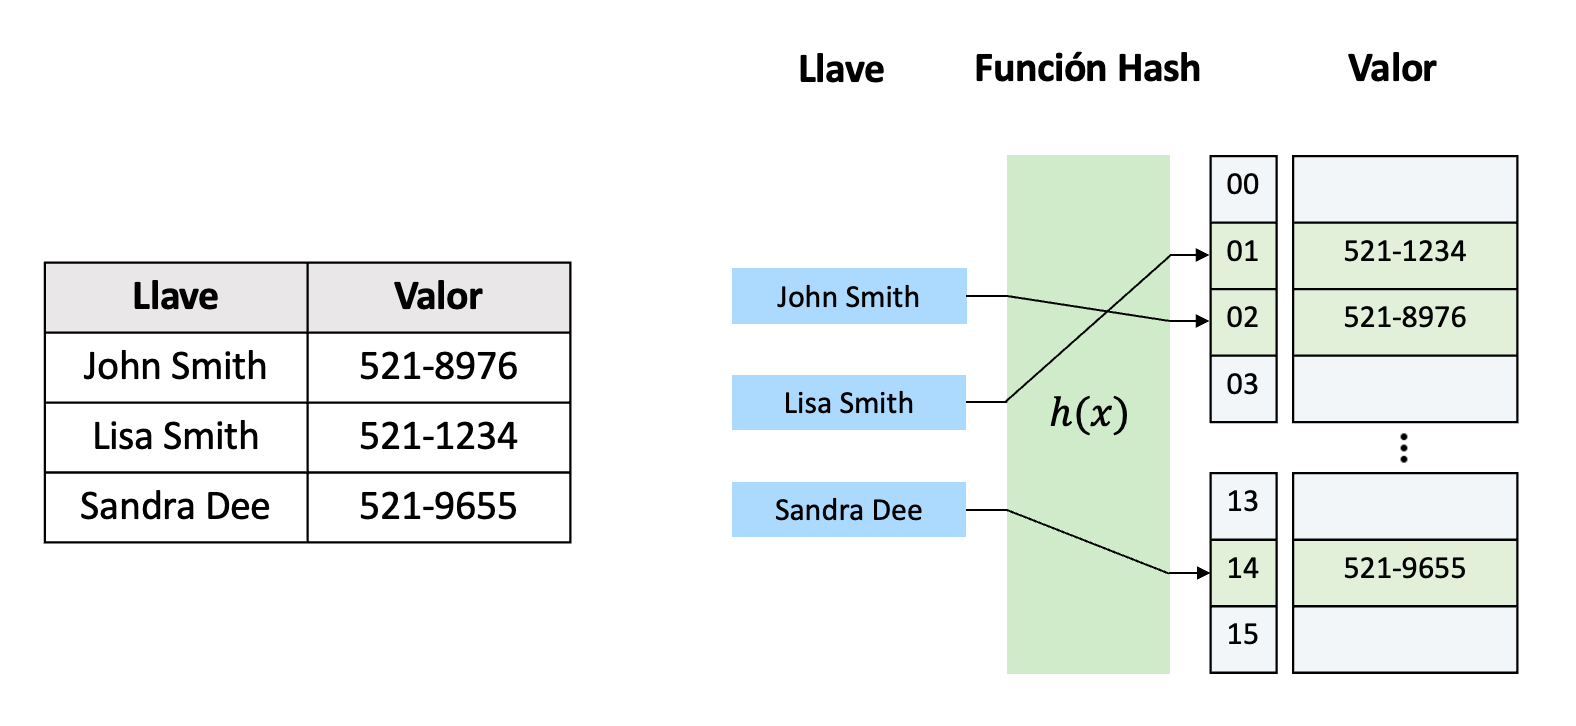
\includegraphics[width=\textwidth]{img/db-example.png}
    \end{block}

    \note<1>{@NOTE x ejemplo:
        \begin{itemize}
            \item referenciar a valores \'unicos
            \item eliminar redundancia en datos repetidos continuamente (Run-Length Encoding)
            \item eliminaci\'on de nulls llevando m\'ascaras de bits, por ejemplo
        \end{itemize}
    }
\end{frame}

\begin{frame}
    \frametitle{Modelo de datos}

    \begin{block}{Restricciones de integridad}
        \begin{itemize}
            \item La llave es un \texttt{string} que debe ser único en la base de datos
            \item El valor es un data arbitrariamente grande, usualmente representado como un \texttt{blob} (\textit{binary large object})
        \end{itemize}

    \end{block}

    \note<1>{@NOTE x ejemplo:
        \begin{itemize}
            \item referenciar a valores \'unicos
            \item eliminar redundancia en datos repetidos continuamente (Run-Length Encoding)
            \item eliminaci\'on de nulls llevando m\'ascaras de bits, por ejemplo
        \end{itemize}
    }
\end{frame}

\begin{frame}
    \frametitle{Modelo de datos}

    \begin{block}{Operaciones}
        Solo se implementan las operaciones básicas soportadas por la estructura de datos.
        \begin{itemize}
            \item \texttt{put(key, value)}: Agregar una llave
            \item \texttt{delete(key)}: Eliminar una llave
            \item \texttt{replace(key)}: Actualizar una llave
            \item \texttt{get(key)}: Buscar una llave 
            \item \texttt{get\_prefix(prefix)}: Buscar las llaves por prefijo  
            \item \texttt{get\_range(key1, key2)}: Buscar un rango de llaves [key1, key2]
        \end{itemize}

        Las operaciones de búsqueda se realizan utilizando comparación lexicográfica.

        

    \end{block}

    \note<1>{@NOTE x ejemplo:
        \begin{itemize}
            \item referenciar a valores \'unicos
            \item eliminar redundancia en datos repetidos continuamente (Run-Length Encoding)
            \item eliminaci\'on de nulls llevando m\'ascaras de bits, por ejemplo
        \end{itemize}
    }
\end{frame}

\begin{frame}
    \frametitle{Consideraciones}

    \begin{table}[h!]
        \centering
        \begin{tabular}{|p{0.45\textwidth}|p{0.45\textwidth}|}
        \hline
        \multicolumn{1}{|c|}{\cellcolor{green1} \textbf{Ventajas}} &  \multicolumn{1}{|c|}{ \cellcolor{red1} \textbf{Desventajas}} \\ \hline
        Altamente eficientes para operaciones de lectura y escritura & Incapacidad de realizar consultas complejas, especialmente con datos interrelacionados \\ \hline
        Flexibilidad para la modelación de datos permitiendo almacenar cualquier tipo de datos como valores & No se asegura el cumplimiento de reglas de negocio sobre los datos almacenados como valores \\ \hline
        Altos niveles de compresión de datos & No soporta operaciones sobre los datos almacenados como valores \\ \hline
        Gran disponibilidad y escalabilidad & No cumple con ACID \\ \hline
        \end{tabular}
    \end{table}

    % \note<2>{@NOTE x ejemplo:
    %     \begin{itemize}
    %         \item referenciar a valores \'unicos
    %         \item eliminar redundancia en datos repetidos continuamente (Run-Length Encoding)
    %         \item eliminaci\'on de nulls llevando m\'ascaras de bits, por ejemplo
    %     \end{itemize}
    % }
\end{frame}


\begin{frame}
    \frametitle{Casos de uso}

    \begin{itemize}
        \item Administración de los datos de sesión de usuarios
        \item Implementación de memorias caché para optimizar el rendimiento de aplicaciones
        \item Almacenamiento de configuraciones de sistemas distribuidos
        \item Sistemas de monitoreo
    \end{itemize}

    % \note<2>{@NOTE x ejemplo:
    %     \begin{itemize}
    %         \item referenciar a valores \'unicos
    %         \item eliminar redundancia en datos repetidos continuamente (Run-Length Encoding)
    %         \item eliminaci\'on de nulls llevando m\'ascaras de bits, por ejemplo
    %     \end{itemize}
    % }
\end{frame}



\begin{frame}
    \frametitle{Implementación de un caso de uso}

    
    \begin{block}{Descripción}
    Un \textit{Domain Name System} (DNS) actúa como una agenda de contactos dentro de Internet, asociando nombres de dominio a direcciones IP. Estos sistemas simplifican el acceso a recursos online mediante el uso de nombres como \texttt{google.com}. 

    \end{block}
    % \note<2>{@NOTE x ejemplo:
    %     \begin{itemize}
    %         \item referenciar a valores \'unicos
    %         \item eliminar redundancia en datos repetidos continuamente (Run-Length Encoding)
    %         \item eliminaci\'on de nulls llevando m\'ascaras de bits, por ejemplo
    %     \end{itemize}
    % }

    \begin{center}
        
        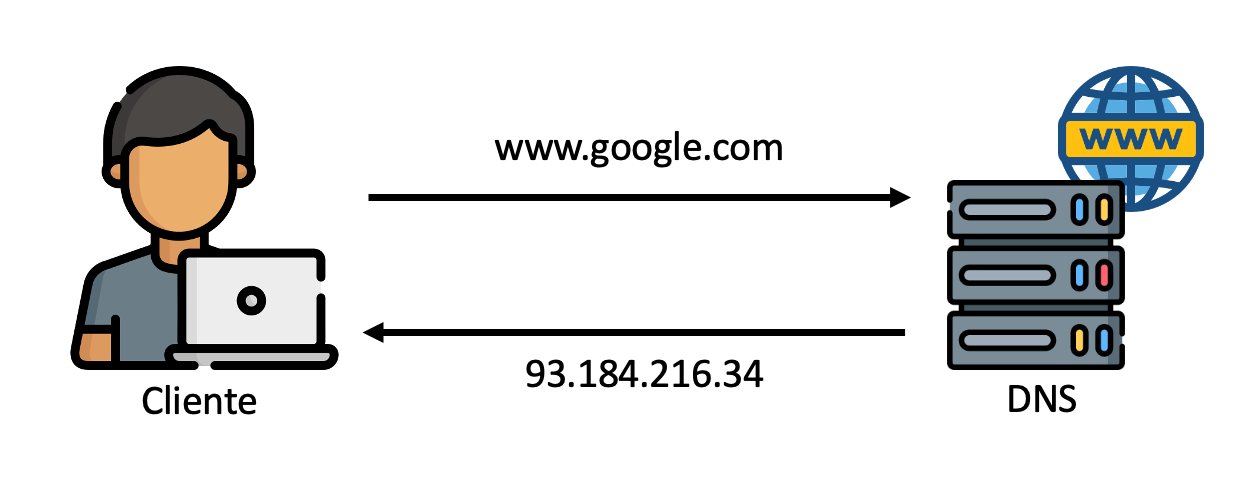
\includegraphics[width=0.6\textwidth]{img/dns.png}
    \end{center}
\end{frame}


\begin{frame}
    \frametitle{Implementación de un caso de uso}

    \begin{block}{Requerimientos}
        \begin{itemize}
            \item \textbf{Simplicidad conceptual}: Solo es necesario almacenar los nombres de dominio y las direcciones IP. Además las consultas se limitan a obtener el IP asociado a un nombre de dominio.
            \item \textbf{Gran volumen de operaciones}: El escenario es muy dinámico, con dispositivos entrando y saliendo de la red mientras se comunican entre sí (es decir, deben de buscar sus IPs).
            \item \textbf{Alta disponibilidad}: La caída de un sistema DNS significaría la interrupción de una gran parte de las comunicaciones en la red, por tanto se debe garantizar la disponibilidad del sistema.
        \end{itemize}

    \end{block}

\end{frame}


\begin{frame}
    \frametitle{Implementación de un caso de uso}

    \begin{block}{Código}
        El código para simular y solucionar el escenario se encuentra en uno de los repositorios
        de la disciplina \href{https://github.com/ISBIG-UH/no-sql-samples/}{https://github.com/ISBIG-UH/no-sql-samples/}

        \begin{center}
            
            
\includegraphics[width=40mm]{img/repo-qrcode.png}
        \end{center}
   
    \end{block}

\end{frame}




    \section{Bases de datos columnares}
    \section{MonetDB}

    \maketitle
\end{document}